\chapter{Numerical Solutions}
As we are usually interested in finding real (or complex) valued solutions of our systems we also have to look into solving them numerically. This chapter focuses on the numerical solution of the mentioned systems.

We will first focus on methods used to solve a more general problem
\begin{align}
	\label{general numerical problem}
	y'(t) &= f(t,y), \quad t \in [t_0, t_l], \\
	y(t_0) &= y_0.
\end{align}


For this we presume that the function $f(t,y)$ is continuous and Lipschitz, thus \emph{Picard-Lindelöf} gives us, that for every $y_0$ it is uniquely solvable in $[t_0, t_l]$.

Numerical Methods work by discretization, this means we divide the time-intervall into

\begin{displaymath}
	t_0 < t_1 < ... < t_N \leq t_l
\end{displaymath}

and consider approximations $y_m \approx y(t_m)$ for $m=1,...,N$. Gitterpunkte, SChrittweite, äquidistant, nicht äquidistant.

\section{Single-Step-Methods}
	The first class of numerical methods we will have a look at are single-step methods. These methods use the previous approximated value $y_j$ and (for implicit methods) also the current approximated value to determine the current value through a \emph{procedural function}. ... waht does implicit and explicit mean?
	
	\begin{definition}
		A numerical method to approximate a differential equation \ref{general numerical problem} on a time-grid $t_0,...,t_l$ with the intermediate values $y_0,...,y_l$ is called a single-step method if it is from the form
		\begin{equation}
			\label{single-step method}
			y_{j+1} = y_j + h_j \phi(t_j,y_j, y_{j+1},h_j).
		\end{equation}
		With the \emph{procedural function} $\phi$. If $\phi$ is not dependent on $y_{j+1}$ then the method is called \emph{explicit}, otherwise it is called \emph{implicit}.
	\end{definition}

	\subsection{Consistency and Convergence}
	
	To compare different single-step methods we have to define some notions to compare their quality. This leads to the definition of the error of the mehtod, its consistency and its convergence.
	
	\begin{definition}
		Let $\tilde{y}_{m+1}$ be the result of one step of \ref{single-step method} with the exact start-vector $y_m = y(t_m)$ then
		\begin{equation}
			\label{local discretization error single step}
			le_{m+1} = le(t_m+h) = y(t_{m+1}) - \tilde{y}_{m+1}, \quad m = 0,...,N-1
		\end{equation}
		is called the \emph{local discretization error} of the single step method at the point $t_{m+1}$.
	\end{definition}

	The error encodes how far off the numerical method is from the true value of the solution. In real applications this solution is usually not known. This shows how important error bounds for numerical methods can be.

	\begin{definition}
		A single-step method is called \emph{consistent} if for all initial value problems \ref{general numerical problem} 
		\begin{equation}
			\lim\limits_{h \to 0} \frac{||le(t+h)||}{h} = 0 \quad \text{for} \quad t_0 \leq t \leq t_l
		\end{equation}
		holds.\newline
		It is called \emph{consistent of order p}, if for a sufficiently smooth function $f$
		\begin{equation}
			||le(t+h)|| \leq Ch^{p+1} \quad \text{for all} \quad h \in \mathopen{(} 0,H \mathclose{]} \quad \text{and} \quad t_0 \leq t \leq t_l - h
		\end{equation}
		holds with $C$ not dependent on $h$.
	\end{definition}

	Consistency aims to give insight in how similar the problem that the numerical methods solves it to the real problem that we want the solution from.

	\begin{definition}
		A single-step method is called \emph{convergent}, if for all initial value problems \ref{general numerical problem} for the \emph{global discretization error}
		\begin{displaymath}
			e_m = y(t_m)-y_h(t_m)
		\end{displaymath}
		holds that
		\begin{displaymath}
			\max\limits_{m}||e_m|| \to 0 \quad \text{for} \quad h_{max} \to 0.
		\end{displaymath}
		The single-step method is called to have the \emph{convergence order} $p$, if
		\begin{displaymath}
			\max\limits_{m} ||e_m|| \leq C h_max^p \quad \text{for} \quad h_{max} \in \mathopen{(} 0,H \mathclose{]} \quad \text{with} \quad t_0 \leq t_m \leq t_l
		\end{displaymath}
		with the constant $C$ not dependent on the step size $h$.
	\end{definition}

	As the name suggestes convergence tries to quantify how far off a numerical solution is from the real solution of a system.

	\subsection{Runge-Kutta Methods}
		A very prevalent family of numerical single-step methods are the \emph{Runge-Kutta} methods. ... Whats the idea behind those methods?
		
		\begin{definition}
			Let $s \in \mathbb{N}$. A single-step method of the form
			\begin{align}
				y_{m+1} = y_m + h \sum_{i=1}^{s} b_i f(t_m + c_ih, y_{m+1}^{(i)}) \\ 
				y_{m+1}^{(i)} = y_m +  \sum_{j=1}^{s} a_{ij} f(t_m + c_jh, y_{m+1}^{(j)})
			\end{align}
			is called a \emph{Runge-Kutta Method} with $s$ steps.
		\end{definition}
		
		We usually collect the coefficients into the vectors and matrices $c=(c_1, ...,c_s)$, $A = (a_{ij})_{ij}$ and $b=(b_1, ..., b_s)$.
		
		If $A$ is a strictly lower triangle matrix, this means for all $j \geq i$ holds $a_{ij} = 0$ then the Runge-Kutta method is explicit, otherwise it is implicit. In general implicit Runge-Kutta methods might need more computational effort because to calculate $y_m^{(i)}$ a nonlinear system of equations has to be solved. But in contrast those methods can also lead to very good stability characteristics.
		
		\begin{lemma}%\cite{NumerikgewöhnlicherDifferentialgleichungen}
			A Runge-Kutta mehtod is consistent, if and only if
			\begin{displaymath}
				\sum_{i=1}^{s} b_i = 1
			\end{displaymath}
		\end{lemma}
		
		The coefficients of a Runge-Kutta method are usually represented in the \emph{Butchertableau}, which was introduced by John C. Butcher and has the following form.
		
		\begin{displaymath}
			\begin{array}{c|ccc}
				c_1 & a_{11} & \dots & a_{1s} \\
				\vdots & \vdots & & \vdots \\
				c_s & a_{s1} & \dots & a_{ss} \\
				\hline
				 & b_1 & \dots & b_s
			\end{array}
			\qquad
			\text{of in matrix form}
			\qquad
			\begin{array}{c|c}
				c & A \\
				\hline
				 & b
			\end{array}
		\end{displaymath}
		
\section{Multistep-Methods}
	based on chapter 4 of book num gew dgl steif nichtsteif \newline
	Linear multistep methods use approxiamtions $u_{m+l}$ along the gridpoints $t_{m+l}, \quad l=0,1,...,k-1$ to calculate the new approximation $u_{m+k}$ at $t_{m+k}$. WE will first discuss topics related to the order of the methods depending on its parameters, stability and convergence.
	
	\begin{definition}
		For given $\alpha_0, ..., \alpha_k$ and $\beta_0, ..., \beta_k$ the iteration rule
		\begin{equation}
			\label{linear-multistep-method}
			\sum_{l=0}^{k} \alpha_l u_{m+l} = h \sum_{l=0}^{k} \beta_l f(t_{m+l}, u_{m+l}), \quad m=0,1,...,N-k
		\end{equation}
		is called a \emph{linear multistep method} (linear k-step method). It is always assumed that $\alpha_k \neq 0$ and $|\alpha_0| + |\beta_k| > 0$. If $\beta_k=0$ holds, then the method is called explicit, otherwise implicit.
	\end{definition}
	
	\begin{figure}[H]
		\centering
		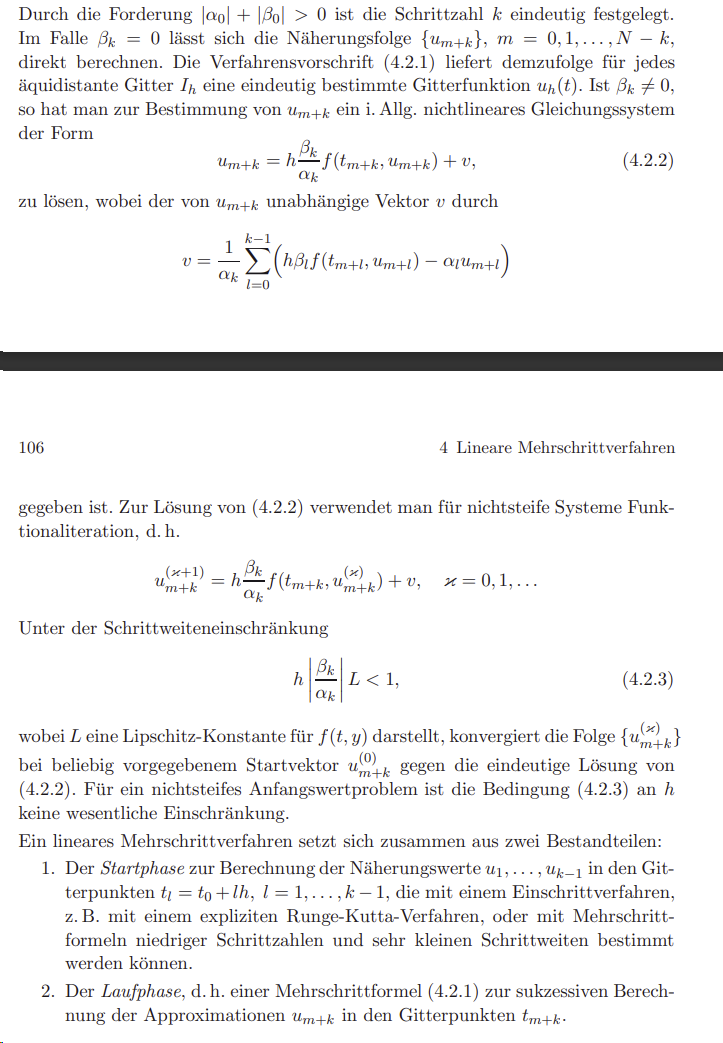
\includegraphics[width=0.7\linewidth]{screenshot010}
		\caption{}
		\label{fig:screenshot010}
	\end{figure}
	
	A linear multi-step method consists of two parts:
	\begin{enumerate}
		\item In the \emph{starting-phase} approximations $u_1,...,u_{k-1}$ for the first $k-1$ gridpoints $t_l = t_0+th, l=1,...,k-1$ are calculated using a single-step method. For example using an explicit Runge-Kutta Methodor a multi-step method with fewer steps.
		
		\item  In the \emph{run-phase} the multi-step formula is used to determine new approximations $u_{m+k}$ for the gridpoint $t_{m+k}$
	\end{enumerate}
	
	For theoretical analysis of the multi-step methods we consider the generating polynomials
	\begin{equation}
		\rho(x) := \sum_{l=0}^{k} \alpha_l x^l
	\end{equation}
	\begin{equation}
		\sigma(x) := \sum_{l=0}^{k} \beta_l x^l
	\end{equation}
	
	\begin{figure}[H]
		\centering
		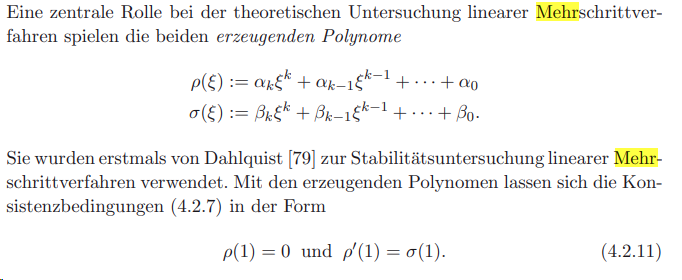
\includegraphics[width=0.7\linewidth]{screenshot013}
		\caption{}
		\label{fig:screenshot013}
	\end{figure}
	
	
	\subsection{Consistency and order}
	local discretization error - def 4.2.2
	\begin{definition}
		Let $\tilde{u}_{m+k}$ be the result of one step of the multi-step method \ref{linear-multistep-method} with the start-vectors $u_m, u_{m+1}, ..., u_{m+k-1}$ lying on the exact solution $y(t)$ of the problem \textbf{reference}. This means
		\begin{displaymath}
			\alpha_k \tilde{u}_{m+k} = \sum_{l=0}^{k-1} \left( h \beta_l f(t_{m+l}, y(t_{m+l})) - \alpha_l y(t_{m+l}) \right) + h \beta_k f(t_{m+k}, \tilde{u}_{m+k}) .
		\end{displaymath}
		Then
		\begin{displaymath}
			le_{m+k} = le(t_{m+k}) = y(t_{m+k}) - \tilde{u}_{m+k}, \quad m=0,1,...,N-k
		\end{displaymath}
		is called the \emph{local discretization error} (local error) of the linear multi-step method \ref{linear-multistep-method} at the point $t_{m+k}$.
	\end{definition}
	
	We will assign the linear difference opreator
	\begin{equation}
		L[y(t),h] = \sum_{l=0}^{k} \left( \alpha_l y(t+lh) - h \beta_l y'(t+lh) \right)
	\end{equation}
	to the local discretization error. Using this we gain the following definition.
	
	\begin{definition}
		A linear multi-step method is called \emph{preconsistent} if for all functions $y(t) \in C^1[t_0,t_l]$
		\begin{displaymath}
			\lim\limits_{h \to 0} L[y(t),h]=0
		\end{displaymath}
		holds. It is called \emph{consistent}, if for all functions $y(t) \in C^2[t_0,t_l]$
		\begin{displaymath}
			\lim\limits_{h \to 0} \frac{1}{h} L[y(t),h] = 0
		\end{displaymath}
		holds. It has the \emph{consistency order p}, if for all functions $y(t) \in C^{p+1}[t_0, t_l]$
		\begin{displaymath}
			L[y(t),h] = \mathcal{O}(h^{p+1}) \quad \text{for} \quad h \to 0
		\end{displaymath}
		holds.
	\end{definition}
	
	\begin{figure}[H]
		\centering
		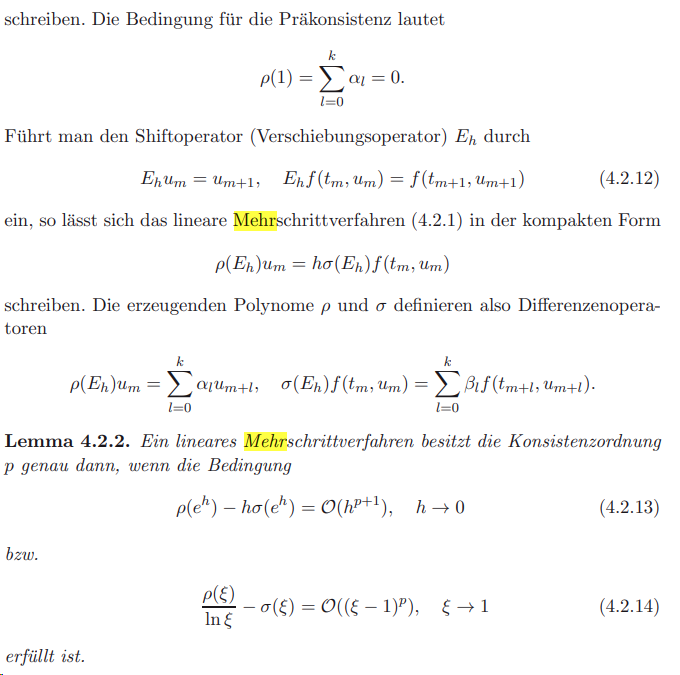
\includegraphics[width=0.7\linewidth]{screenshot014}
		\caption{}
		\label{fig:screenshot014}
	\end{figure}
	
	
	
	\subsection{Convergence and stability}
	
	\begin{definition}
		A linear multi-step method is called \emph{zero-stable} if all solutions of the difference equation
		\begin{displaymath}
			\sum_{l=0}^{k} \alpha_l u_{m+l} = 0
		\end{displaymath}
		are bounded.
	\end{definition}
	
	\begin{theorem}
		A linear multi-step method is zero-stable, if and only if the polynomial $\rho(x)$ fullfills the root-condition, this means:
		\begin{enumerate}
			\item All roots $\bar{x}$ of $\rho(x)$ are within the unit-circle $|\bar{x}| \leq$ in the complex plane.
			\item All roots $\bar{x}$ with $|x| = 1$ are singular.
		\end{enumerate}
	\end{theorem}
	
	
	\textbf{from circuit book below, above from modelling book}

\section{Implicit linear multi-step formulas}
These kinds of multi-step methods are conventionally used to numerically solve the systems obtained using modified nodal analysis. 

The conventional approach can be split into three main steps:
\begin{enumerate}
	\item Computation of consistent initial values
	\item numerical integration based on multi-step schemes
	\item transformation of the DAE into a nonlinear system and its numerical solutioon by Newton's procedure (?????????????????will not be discussed further because not very specific)
\end{enumerate}

\textbf{Consistant initial values} 
\begin{figure}[H]
	\centering
	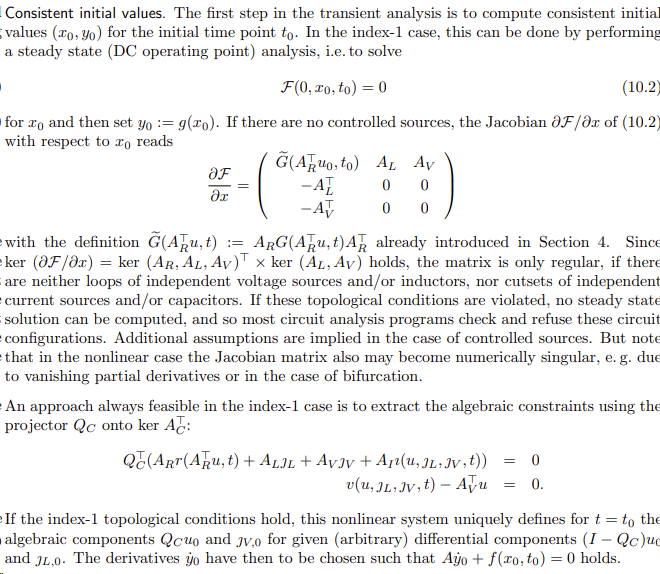
\includegraphics[width=0.7\linewidth]{screenshot009}
	\caption{}
	\label{fig:screenshot009}
\end{figure}

\textbf{Nunmerical integration}.


\subsection{BDF schemes and trapezoidal rule}